%%==================================================================%%
%% Author : Abascal Fernández, Patricia                             %%
%%          Sánchez Barreiro, Pablo                                 %%
%% Version: 1.0, 15/04/2013                                         %%
%%                                                                  %%
%% Memoria del Proyecto Fin de Carrera                              %%
%% Background/Slicer Pattern                                        %%
%===================================================================%%
Antes de proceder a la explicación del Patrón Slicer, es conveniente presentar el concepto de Clase Parcial C\# de manera breve al lector. Las clases parciales C\#~\cite{albahari:2010} permiten dividir la implementación de una clase en varios archivos de código fuente. Cada fragmento representa una parte de la funcionalidad global de la clase. Todos estos fragmentos se combinan en tiempo de compilación para crear una única clase, la cual contiene toda la funcionalidad especificada en las clases parciales. Por lo tanto, las clases parciales C\# parecen un mecanismo adecuado para implementar características, tal como ha sido identificado por diversos autores~\cite{laguna:2007,laguna:2010}, dado que cada incremento en funcionalidad perteneciente a una característica se podría encapsular en una clase parcial separada. Sin embargo, las clases parciales tiene un serio inconveniente para ser utilizadas como un mecanismo de apoyo a la orientación de características: no son compatibles con la extensión de métodos ni la reescritura. El Patrón Slicer surge como patrón para solución de esta limitación.

El problema a solucionar por el Patrón Slicer tiene su origen en el hecho de que no se puede disponer de métodos con el mismo nombre en diferentes clases parciales.

La instanciación del Patrón Slicer en los métodos regulares, consiste en añadir un prefijo a cada método que se corresponda con el nombre de la característica a la que cada método pertenece. La Figura~\ref{back:fig:slicerPattern} ilustra cómo el caso de estudio de Hogar Inteligente ha sido refactorizado siguiendo dicha idea. En esta figura, las características han sido representadas como rectángulos conteniendo clases. Cada rectángulo ha sido etiquetado con el nombre de la característica que representa.

\begin{figure}[!tb]
  \centering
	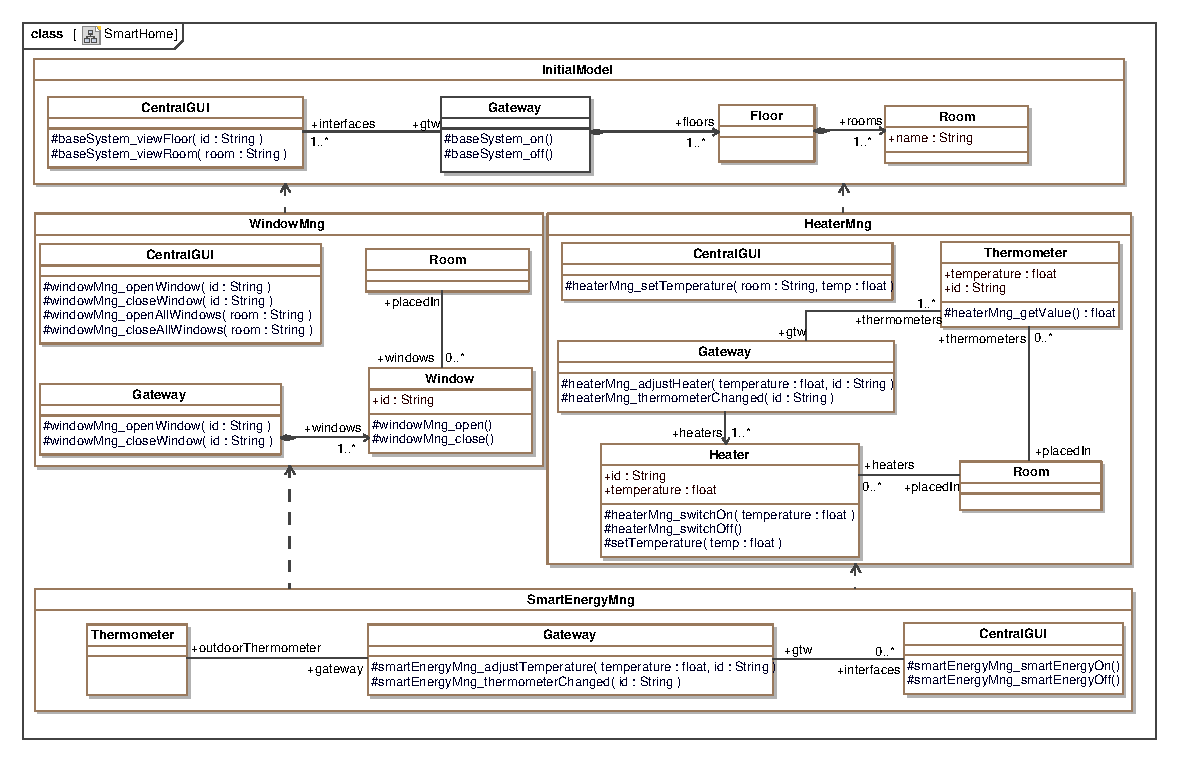
\includegraphics[width=.95\linewidth]{background/images/slicerPattern.eps} \\
  \caption{Proceso de Desarrollo de una Línea de Productos Software}
  \label{back:fig:slicerPattern}
\end{figure}

Usando esta estrategia se puede comprobar cómo, por ejemplo, las versiones del método \emph{thermometerChanged} correspondientes a las características \emph{HeaterMng} y \emph{SmartEnergyMng} han sido transformadas en \emph{heaterMng_thermometerChanged} y \emph{smartEnergyMng_thermometerChanged} respectivamente y por tanto pueden co-existir sin que sus nombres colisionen. Es más, el método \emph{smartEnergyMng_thermometerChanged} puede extender del método \emph{heaterMng_thermometerChanged}. Se dispone por tanto de varias versiones parciales de un mismo método.

Para generar un producto específico es necesario que, a nivel de Ingeniería de Aplicación, se cree la denominada "versión limpia" del método \emph{thermometerChanged}, es decir, sin el prefijo. Mientras que las versiones de dicho método creadas en el nivel de Ingeniería del Dominio que han sido prefijadas con el nombre de la característica a la que cada método pertenece pasarán a ser denominadas "versiones sucias" de dicho método. Además, para asegurar que se invoca la versión correcta del método, no se deberían poder invocar los métodos \emph{heaterMng_thermometerChanged} y \emph{smartEnergyMng_thermometerChanged} directamente y por dicha razón todas las versiones sucias de los métodos son privadas. De dicha forma los objetos de las demás clases sólo podrán invocar a la versión limpia del método y dicha versión, redireccionará la llamada a las versiones sucias de los métodos correspondientes de acuerdo a las características seleccionadas.

Sin embargo este patrón no puede ser utilizado para los constructores de la clase ya que los constructores no se pueden renombrar porque deben tener un nombre específico. De esta forma, la instanciación del Patrón Slicer en los constructores se realiza de forma diferente a la instanciación del resto de métodos. De esta forma, cada clase parcial X correspondiente a una caracterísica F tendrá un método privado llamado <F>\_init\_<X> que contendrá el fragmento de la lógica del constructor correspondiente a la característica F.

La Figura~\ref{back:code:constSlicerPattern} muestra cómo se aplica dicha técnica. Se puede apreciar cómo la lógica del constructor para \emph{Gateway} ha sido encapsulada en un método llamado  \emph{baseSystem\_initGateway} (Figura~\ref{back:code:constSlicerPattern} líneas 03-06). La misma técnica ha sido usada en la Figura~\ref{back:code:constSlicerPattern} líneas 10-12 con la característica \emph{WindowMng}. El siguiente paso es encontrar un mecanismo que permita componer dichos fragmentos de acuerdo a una selección de  características dada, de esta forma, como se puede apreciar en la Figura~\ref{back:code:constSlicerPattern} líneas 16-20, el constructor para la clase Gateway es creado con las características seleccionadas por el usuario final, en el caso analizado, por ejemplo, solo se ha seleccionado la característica \emph{WindowMng}.

\begin{figure}[tb!]
\begin{center}
\begin{footnotesize}
\begin{verbatim}
File BaseSystem/Gateway.cs
--------------------------------------------------------
01 public partial class Gateway {
02      ...
03      private void BaseSystem_initGateway() {
04          this.floors = new List<Floors>();
05          this.interfaces = new List<CentralGUI>();
06      }
07 }

File WindowMng/Gateway.cs
--------------------------------------------------------
08 public partial class Gateway {
09      ...
10      private windowMng_initGateway() {
11          this.windows = new List<Window>();
12      }
13 }

File MyHouse/Gateway.cs
--------------------------------------------------------
14 public partial class Gateway {
15      ...
16      public Gateway() {
17          // WindowMng has been selected
18          baseSystem_initGateway();
19          windowMng_initGateway();
20      }
21 }
\end{verbatim}
\end{footnotesize}
\end{center}
\caption{Código para el constructor de la clase Gateway usando clases parciales y patrón slicer}
\label{back:code:constSlicerPattern}
\end{figure}

Concluyendo con el Patrón Slicer, tanto los métodos regulares como con los constructores pueden ser extendidos y reescritos usando dicho patrón y solucionando así las limitaciones ofrecidas por el uso de clases parciales como mecanismo de soporte orientado a características.
